\documentclass[a4paper]{article}
\usepackage[margin=1.0in]{geometry}
\usepackage{longtable}
\usepackage{graphicx}
\usepackage{grffile}

\title{Metabolomic Data Analysis with MetaboAnalyst 6.0}
\author{ Name: guest2805454613693819169 }
\usepackage{Sweave}
\begin{document}
\parskip=.3cm
\maketitle
\section{Background}
 The Pathway Analysis module combines results from powerful pathway  enrichment analysis with pathway topology analysis to help researchers identify the most relevant pathways involved in the conditions under study. 

 There are many commercial pathway analysis software tools such as Pathway Studio, MetaCore, or Ingenuity Pathway Analysis (IPA), etc. Compared to these commercial tools, the pathway analysis module was specifically developed  for metabolomics studies. It uses high-quality KEGG metabolic pathways as the backend knowledgebase.  This module integrates many well-established (i.e. univariate analysis, over-representation analysis) methods, as well as novel algorithms and concepts (i.e. Global Test, GlobalAncova, network topology analysis) into pathway analysis. Another feature is a Google-Map style interactive visualization system to deliver  the analysis results in an intuitive manner.
\section{Data Input}
 The Pathway Analysis module accepts either a list of compound labels (common names, HMDB IDs or KEGG IDs) with one compound per row,  or a compound concentration table with samples in rows and compounds in columns. The second column must be  phenotype labels (binary, multi-group, or continuous). The table is uploaded as comma separated values (.csv). 

\section{Compound Name Matching}

The first step is to standardize the compound labels used in user uploaded data. This is a necessary step since
these compounds will be subsequently compared with compounds contained in the pathway library.
There are three outcomes from the step - exact match, approximate match (for common names only), and no match.
Users should click the textbf{View} button from the approximate matched results to manually select the correct one.
Compounds without match will be excluded from the subsequently pathway analysis.



\textbf{Table 1} shows the conversion results. Note: \textit{1} indicates exact match, \textit{2}
indicates approximate match, and \textit{0} indicates no match. A text file contain the result can be
found the downloaded file \textit{name\_map.csv}


% latex table generated in R 4.3.2 by xtable 1.8-4 package
% Fri Jan  5 13:58:58 2024
\begingroup\scriptsize
\begin{longtable}{rlllllll}
\caption{Result from Compound Name Mapping} \\ 
  \hline
 & Query & Match & HMDB & PubChem & KEGG & SMILES & Comment \\ 
  \hline
1 & 1-stearoyl-2-oleoyl-GPG (18:0/18:1) & NA & NA & NA & NA & NA & 0 \\ 
  2 & hydroxyproline & 4-Hydroxyproline & HMDB0000725 & 5810 & C01157 & O[C@H]1CN[C@@H](C1)C(O)=O & 1 \\ 
  3 & N-acetylphenylalanine & N-Acetyl-L-phenylalanine & HMDB0000512 & 74839 & C03519 & CC(=O)N[C@@H](CC1=CC=CC=C1)C(O)=O & 1 \\ 
  4 & 2-phosphoglycerate & 2-Phosphoglyceric acid & HMDB0000362 & 59 &  & OCC(OP(O)(O)=O)C(O)=O & 1 \\ 
  5 & nervonoylcarnitine (C24:1) & NA & NA & NA & NA & NA & 0 \\ 
  6 & butyrylcarnitine (C4) & NA & NA & NA & NA & NA & 0 \\ 
  7 & homostachydrine & Proline betaine & HMDB0004827 & 115244 & C10172 & C[N+]1(C)CCC[C@H]1C([O-])=O & 1 \\ 
  8 & acetyl-CoA & Acetyl-CoA & HMDB0001206 & 444493 & C00024 & CC(=O)SCCNC(=O)CCNC(=O)[C@H](O)C(C)(C)COP(O)(=O)OP(O)(=O)OC[C@H]1O[C@H]([C@H](O)[C@@H]1OP(O)(O)=O)N1C=NC2=C1N=CN=C2N & 1 \\ 
  9 & homoarginine & Homo-L-arginine & HMDB0000670 & 9085 & C01924 & N[C@@H](CCCCNC(N)=N)C(O)=O & 1 \\ 
  10 & 1-stearoyl-GPG (18:0) & NA & NA & NA & NA & NA & 0 \\ 
  11 & 1-stearoyl-2-arachidonoyl-GPI (18:0/20:4) & NA & NA & NA & NA & NA & 0 \\ 
  12 & pyridoxate & 4-Pyridoxic acid & HMDB0000017 & 6723 & C00847 & CC1=NC=C(CO)C(C(O)=O)=C1O & 1 \\ 
  13 & 1-stearoyl-2-oleoyl-GPE (18:0/18:1) & NA & NA & NA & NA & NA & 0 \\ 
  14 & 2-hydroxystearate & 2-Hydroxystearic acid & HMDB0062549 & 439887 & C03045 & CCCCCCCCCCCCCCCC[C@H](O)C(O)=O & 1 \\ 
  15 & N-acetylmethionine sulfoxide & N-Acetylmethionine sulfoxide & HMDB0240343 & 7408371 &  & CC(=O)N[C@@H](CCS(C)=O)C(O)=O & 1 \\ 
  16 & NADH & NADH & HMDB0001487 & 439153 & C00004 & NC(=O)C1=CN(C=CC1)[C@@H]1O[C@H](COP(O)(=O)OP(O)(=O)OC[C@H]2O[C@H]([C@H](O)[C@@H]2O)N2C=NC3=C2N=CN=C3N)[C@@H](O)[C@H]1O & 1 \\ 
  17 & pentadecanoate (15:0) & NA & NA & NA & NA & NA & 0 \\ 
  18 & leucylglycine & Glycylleucine & HMDB0000759 & 92843 & C02155 & CC(C)C[C@H](NC(=O)CN)C(O)=O & 1 \\ 
  19 & 1-stearoyl-2-dihomo-linolenoyl-GPI (18:0/20:3n3 or 6) & NA & NA & NA & NA & NA & 0 \\ 
  20 & argininosuccinate & Argininosuccinic acid & HMDB0000052 & 16950 & C03406 & N[C@@H](CCCNC(=N)N[C@@H](CC(O)=O)C(O)=O)C(O)=O & 1 \\ 
  21 & X-10445 & NA & NA & NA & NA & NA & 0 \\ 
  22 & 3-hydroxyhexanoate & (R)-3-Hydroxyhexanoic acid & HMDB0010718 & 10197713 &  & CCC[C@@H](O)CC(O)=O & 1 \\ 
  23 & ergothioneine & Ergothioneine & HMDB0003045 & 5351619 & C05570 & C[N+](C)(C)[C@@H](CC1=CNC(=S)N1)C([O-])=O & 1 \\ 
  24 & thiamin monophosphate & Thiamine monophosphate & HMDB0002666 & 1131 & C01081 & CC1=C(CCOP(O)(O)=O)SC=[N+]1CC1=CN=C(C)N=C1N & 1 \\ 
  25 & N1-methyl-4-pyridone-3-carboxamide & N1-Methyl-4-pyridone-3-carboxamide & HMDB0004194 & 440810 & C05843 & CN1C=CC(=O)C(=C1)C(N)=O & 1 \\ 
  26 & 1-margaroylglycerol (17:0) & NA & NA & NA & NA & NA & 0 \\ 
  27 & methionine sulfone & Methionine sulfone & HMDB0062174 & 445282 &  & CS(=O)(=O)CC[C@H](N)C(O)=O & 1 \\ 
  28 & butenoylcarnitine (C4:1) & NA & NA & NA & NA & NA & 0 \\ 
  29 & AICA ribonucleotide & AICAR & HMDB0001517 & 65110 & C04677 & NC(=O)C1=C(N)N(C=N1)[C@@H]1O[C@H](COP(O)(O)=O)[C@@H](O)[C@H]1O & 1 \\ 
  30 & oxindolylalanine & NA & NA & NA & NA & NA & 0 \\ 
  31 & 5,6-dihydrouridine & 5,6-Dihydrouridine & HMDB0000497 & 94312 &  & OC[C@H]1O[C@H]([C@H](O)[C@@H]1O)N1CCC(=O)NC1=O & 1 \\ 
  32 & arachidate (20:0) & NA & NA & NA & NA & NA & 0 \\ 
  33 & 1-arachidonoyl-GPC (20:4n6) & NA & NA & NA & NA & NA & 0 \\ 
  34 & N-acetylthreonine & N-Acetylthreonine & HMDB0062557 & 152204 &  & C[C@@H](O)[C@H](NC(C)=O)C(O)=O & 1 \\ 
  35 & xanthine & Xanthine & HMDB0000292 & 1188 & C00385 & O=C1NC2=C(NC=N2)C(=O)N1 & 1 \\ 
  36 & sphingomyelin (d18:2/21:0, d16:2/23:0) & NA & NA & NA & NA & NA & 0 \\ 
  37 & AMP & Adenosine monophosphate & HMDB0000045 & 6083 & C00020 & NC1=C2N=CN([C@@H]3O[C@H](COP(O)(O)=O)[C@@H](O)[C@H]3O)C2=NC=N1 & 1 \\ 
  38 & NADHX & NADHX & HMDB0059644 & 440516 & C04856 & NC(=O)C1=CN([C@@H]2O[C@H](COP(O)(=O)OP(O)(=O)OC[C@H]3O[C@H]([C@H](O)[C@@H]3O)N3C=NC4=C(N)N=CN=C34)[C@@H](O)[C@H]2O)[C@@H](O)CC1 & 1 \\ 
  39 & N-monomethylarginine & NA & NA & NA & NA & NA & 0 \\ 
  40 & 1-palmitoyl-2-linoleoyl-GPE (16:0/18:2) & NA & NA & NA & NA & NA & 0 \\ 
  41 & oleoylcholine & Oleoylcholine & HMDB0240596 & 59040790 &  & CCCCCCCC$\backslash$C=C/CCCCCCCC(=O)OCC[N+](C)(C)C & 1 \\ 
  42 & 2-hydroxydecanoate & 2-Hydroxydecanoate & HMDB0094656 & 5312797 &  & CCCCCCCC[C@H](O)C(O)=O & 1 \\ 
  43 & heptadecasphingosine (d17:1) & NA & NA & NA & NA & NA & 0 \\ 
  44 & docosapentaenoate (n6 DPA; 22:5n6) & NA & NA & NA & NA & NA & 0 \\ 
  45 & proline & Proline & HMDB0000162 & 145742 & C00148 & OC(=O)[C@@H]1CCCN1 & 1 \\ 
  46 & 1-stearoyl-2-arachidonoyl-GPS (18:0/20:4) & NA & NA & NA & NA & NA & 0 \\ 
  47 & 1-linoleoyl-2-linolenoyl-GPC (18:2/18:3) & NA & NA & NA & NA & NA & 0 \\ 
  48 & 4-hydroxyglutamate & 4-Hydroxy-L-glutamic acid & HMDB0002273 & 440854 & C05947 & N[C@@H](C[C@@H](O)C(O)=O)C(O)=O & 1 \\ 
  49 & 3-hydroxy-2-ethylpropionate & 2-Ethylhydracrylic acid & HMDB0000396 & 188979 &  & CCC(CO)C(O)=O & 1 \\ 
  50 & stearoylcarnitine (C18) & NA & NA & NA & NA & NA & 0 \\ 
  51 & glutarate (C5-DC) & NA & NA & NA & NA & NA & 0 \\ 
  52 & X-26107 & NA & NA & NA & NA & NA & 0 \\ 
  53 & 1-palmityl-GPE (O-16:0) & NA & NA & NA & NA & NA & 0 \\ 
  54 & S-methylglutathione & NA & NA & NA & NA & NA & 0 \\ 
  55 & ophthalmate & Ophthalmic acid & HMDB0005765 & 7018721 & C21016 & CC[C@H](NC(=O)CC[C@H](N)C(O)=O)C(=O)NCC(O)=O & 1 \\ 
  56 & butyrate/isobutyrate (4:0) & NA & NA & NA & NA & NA & 0 \\ 
  57 & CDP-choline & Citicoline & HMDB0001413 & 13805 & C00307 & C[N+](C)(C)CCOP(O)(=O)OP(O)(=O)OC[C@H]1O[C@H]([C@H](O)[C@@H]1O)N1C=CC(N)=NC1=O & 1 \\ 
  58 & ribonate & Ribonic acid & HMDB0000867 & 5460677 & C01685 & OC[C@@H](O)[C@@H](O)[C@@H](O)C(O)=O & 1 \\ 
  59 & 2-myristoyl-GPC (14:0) & NA & NA & NA & NA & NA & 0 \\ 
  60 & methylphosphate & Methylphosphate & HMDB0061711 & 13130 &  & COP(O)(O)=O & 1 \\ 
  61 & lactate & Lactic acid & HMDB0000190 & 107689 & C00186 & C[C@H](O)C(O)=O & 1 \\ 
  62 & 2-palmitoyl-GPC (16:0) & NA & NA & NA & NA & NA & 0 \\ 
  63 & anserine & Anserine & HMDB0000194 & 112072 & C01262 & CN1C=NC=C1C[C@H](NC(=O)CCN)C(O)=O & 1 \\ 
  64 & ethylmalonate & Ethylmalonic acid & HMDB0000622 & 11756 &  & CCC(C(O)=O)C(O)=O & 1 \\ 
  65 & 1-palmityl-GPC (O-16:0) & NA & NA & NA & NA & NA & 0 \\ 
  66 & methyl glucopyranoside (alpha + beta) & NA & NA & NA & NA & NA & 0 \\ 
  67 & 4-imidazoleacetate & Imidazoleacetic acid & HMDB0002024 & 96215 & C02835 & OC(=O)CC1=CN=CN1 & 1 \\ 
  68 & creatine phosphate & Phosphocreatine & HMDB0001511 & 587 & C02305 & CN(CC(O)=O)C(=N)NP(O)(O)=O & 1 \\ 
  69 & 13-HODE + 9-HODE & NA & NA & NA & NA & NA & 0 \\ 
  70 & hippurate & Hippuric acid & HMDB0000714 & 464 & C01586 & OC(=O)CNC(=O)C1=CC=CC=C1 & 1 \\ 
  71 & biopterin & Biopterin & HMDB0000468 & 445040 & C06313 & C[C@H](O)[C@H](O)C1=CNC2=NC(N)=NC(=O)C2=N1 & 1 \\ 
  72 & phytosphingosine & Phytosphingosine & HMDB0004610 & 122121 & C12144 & CCCCCCCCCCCCCC[C@@H](O)[C@@H](O)[C@@H](N)CO & 1 \\ 
  73 & 1-adrenoyl-GPC (22:4) & NA & NA & NA & NA & NA & 0 \\ 
  74 & palmitoylcholine & Palmitoylcholine & HMDB0240592 & 151731 &  & CCCCCCCCCCCCCCCC(=O)OCC[N+](C)(C)C & 1 \\ 
  75 & N,N,N-trimethyl-5-aminovalerate & NA & NA & NA & NA & NA & 0 \\ 
  76 & acetylcholine & Acetylcholine & HMDB0000895 & 187 & C01996 & CC(=O)OCC[N+](C)(C)C & 1 \\ 
  77 & myristate (14:0) & NA & NA & NA & NA & NA & 0 \\ 
  78 & 1-arachidonoyl-GPE (20:4n6) & NA & NA & NA & NA & NA & 0 \\ 
  79 & 1-stearoyl-2-dihomo-linolenoyl-GPS (18:0/20:3n3 or 6) & NA & NA & NA & NA & NA & 0 \\ 
  80 & 1-pentadecanoyl-2-linoleoyl-GPC (15:0/18:2) & NA & NA & NA & NA & NA & 0 \\ 
  81 & sphingomyelin (d18:1/24:1, d18:2/24:0) & NA & NA & NA & NA & NA & 0 \\ 
  82 & 2-hydroxyadipate & 2-Hydroxyadipic acid & HMDB0000321 & 193530 & C02360 & OC(CCCC(O)=O)C(O)=O & 1 \\ 
  83 & UDP-galactose & Uridine diphosphategalactose & HMDB0000302 & 18068 & C00052 & OC[C@H]1O[C@H](OP(O)(=O)OP(O)(=O)OC[C@H]2O[C@H]([C@H](O)[C@@H]2O)N2C=CC(=O)NC2=O)[C@H](O)[C@@H](O)[C@H]1O & 1 \\ 
  84 & linoleoyl ethanolamide & Linoleoyl ethanolamide & HMDB0012252 & 5283446 &  & CCCCC$\backslash$C=C/C$\backslash$C=C/CCCCCCCC(=O)NCCO & 1 \\ 
  85 & 1,2-distearoyl-GPC (18:0/18:0) & NA & NA & NA & NA & NA & 0 \\ 
  86 & behenoyl sphingomyelin (d18:1/22:0) & NA & NA & NA & NA & NA & 0 \\ 
  87 & dihomo-linoleoylcarnitine (C20:2) & NA & NA & NA & NA & NA & 0 \\ 
  88 & phenylalanylalanine & Phenylalanylalanine & HMDB0028988 & 5488196 &  & C[C@H](NC(=O)[C@@H](N)CC1=CC=CC=C1)C(O)=O & 1 \\ 
  89 & 2-aminoheptanoate & 2-Aminoheptanoate & HMDB0094649 & 5312965 &  & CCCCC[C@H](N)C(O)=O & 1 \\ 
  90 & 1-palmitoyl-GPC (16:0) & NA & NA & NA & NA & NA & 0 \\ 
  91 & ethyl beta-glucopyranoside & NA & NA & NA & NA & NA & 0 \\ 
  92 & ceramide (d18:1/20:0, d16:1/22:0, d20:1/18:0) & NA & NA & NA & NA & NA & 0 \\ 
  93 & 3-hydroxybutyrate (BHBA) & NA & NA & NA & NA & NA & 0 \\ 
  94 & X-12100 & NA & NA & NA & NA & NA & 0 \\ 
  95 & tetradecanedioate (C14) & NA & NA & NA & NA & NA & 0 \\ 
  96 & 1,2-dilinolenoyl-GPC (18:3/18:3) & NA & NA & NA & NA & NA & 0 \\ 
  97 & maltotriose & Maltotriose & HMDB0001262 & 439586 & C01835 & OC[C@H]1O[C@H](O[C@H]2[C@H](O)[C@@H](O)[C@@H](O[C@H]3[C@H](O)[C@@H](O)C(O)O[C@@H]3CO)O[C@@H]2CO)[C@H](O)[C@@H](O)[C@@H]1O & 1 \\ 
  98 & butyryl/isobutyryl CoA & NA & NA & NA & NA & NA & 0 \\ 
  99 & adrenate (22:4n6) & NA & NA & NA & NA & NA & 0 \\ 
  100 & 2S,3R-dihydroxybutyrate & NA & NA & NA & NA & NA & 0 \\ 
   \hline
\hline
\end{longtable}
\endgroup\clearpage


\section{Pathway Analysis}

In this step, users are asked to select a pathway library, as well as specify the algorithms for pathway
enrichment analysis and pathway topology analysis. 

\subsection{Pathway Library}

There are 15 pathway libraries currently supported, with a total of 1173 pathways :

\begin{itemize}
\item{Homo sapiens (human) [80]}
\item{Mus musculus (mouse) [82]}
\item{Rattus norvegicus (rat) [81]}
\item{Bos taurus (cow) [81]}
\item{Danio rerio (zebrafish) [81]}
\item{Drosophila melanogaster (fruit fly) [79]}
\item{Caenorhabditis elegans (nematode) [78]}
\item{Saccharomyces cerevisiae (yeast) [65]}
\item{Oryza sativa japonica (Japanese rice) [83]}
\item{Arabidopsis thaliana (thale cress) [87]}
\item{Escherichia coli K-12 MG1655 [87]}
\item{Bacillus subtilis [80]}
\item{Pseudomonas putida KT2440 [89]}
\item{Staphylococcus aureus N315 (MRSA/VSSA)[73]}
\item{Thermotoga maritima [57]}
\end{itemize}



Your selected pathway library code is \textbf{ mmu }(KEGG organisms abbreviation).


\subsection{Over Representation Analysis}

Over-representation analysis tests if a particular group of compounds
is represented more than expected by chance within the user uploaded compound
list. In the context of pathway analysis, we are testing if compounds involved
in a particular pathway are enriched compared to random hits. MetPA offers two of the
most commonly used methods for over-representation analysis: 

\begin{itemize}
\item{Fishers'Exact test}
\item{Hypergeometric Test}
\end{itemize}
\textit{Please note, MetPA uses one-tailed Fisher's exact test which will give essentially
the same result as the result calculated by the hypergeometric test.}






\subsection{Pathway Topology Analysis}

The structure of biological pathways represent our knowledge about the complex relationships among molecules
within a cell or a living organism. However, most pathway analysis algorithms fail to take structural information
into consideration when estimating which pathways are significantly changed under conditions of study. 
It is well-known that changes in more important positions of a network will trigger a more severe
impact on the pathway than changes occurred in marginal or relatively isolated positions.



The pathway topology analysis uses two well-established node centrality measures to estimate node importance - \textbf{degree centrality}
and \textbf{betweenness centrality}. Degree centrality is defined as the number of links occurred upon a node.
For a directed graph there are two types of degree: in-degree for links come from other nodes, and out-degree
for links initiated from the current node. Metabolic networks are directed graph. Here we only consider the
out-degree for node importance measure. It is assumed that nodes upstream will have regulatory roles for
the downstream nodes, not vice versa. The betweenness centrality measures the number of shortest paths going
through the node. Since the metabolic network is directed, we use the relative betweenness centrality for a metabolite
as the importance measure. The degree centrality measure focuses more on local connectivities, while the betweenness
centrality measure focuses more on global network topology. For more detailed discussions on various graph-based
methods for analyzing biological networks, please refer to the article by Tero Aittokallio, T. et al.
\footnote{Tero Aittokallio and Benno Schwikowski. \textit{Graph-based methods for analyzing networks in cell biology},
Briefings in Bioinformatics 2006 7(3):243-255}



\textit{Please note, for comparison among different pathways, the node importance values calculated from centrality measures
are further normalized by the sum of the importance of the pathway. Therefore, the total/maximum importance of each pathway
is 1; the importance measure of each metabolite node is actually the percentage w.r.t the total pathway importance,
and the pathway impact value is the cumulative percentage from the matched metabolite nodes.}





\section{Pathway Analysis Result}

The results from pathway analysis are presented graphically as well as in a detailed table.



A Google-map style interactive visualization system was implemented to facilitate data exploration.
The graphical output contains three levels of view: \textbf{metabolome view}, \textbf{pathway view},
and \textbf{compound view}. Only the metabolome view is shown below.
Pathway views and compound views are generated dynamically based on your interactions with the
visualization system. They are available in your downloaded files. 

\begin{figure}[htp]
\begin{center}
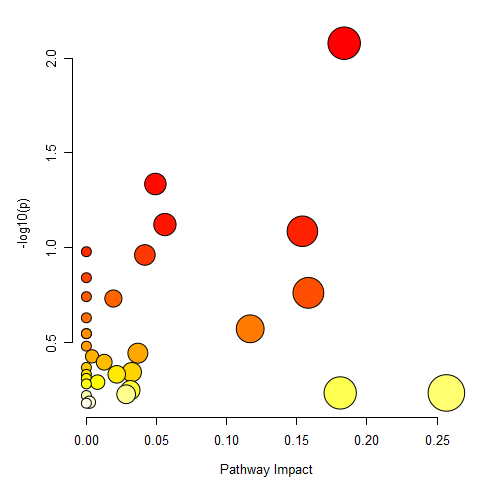
\includegraphics[width=1.0\textwidth]{path_view_0_dpi72.png}
\caption{Summary of Pathway Analysis}
\end{center}
\label{path_view_0_dpi72.png}
\end{figure}
\clearpage


The table below shows the detailed results from the pathway analysis. Since
we are testing many pathways at the same time, the statistical p values from
enrichment analysis are further adjusted for multiple testings. In particular, 
the \textbf{Total} is the total number of compounds in the pathway;
the \textbf{Hits} is the actually matched number from the user uploaded data;
the \textbf{Raw p} is the original p value calculated from the enrichment analysis;
the \textbf{Holm p} is the p value adjusted by Holm-Bonferroni method;
the \textbf{FDR p} is the p value adjusted using False Discovery Rate;
the \textbf{Impact} is the pathway impact value calculated from pathway topology analysis.


